\section{RL Agents and Results}

\subsection{Algorithms and Training}

PPO~\cite{schulman2017ppo} handles the eight-group \texttt{MultiDiscrete} action space ($26^8$ joint actions); DQN~\cite{mnih2015dqn} is practical only for the single-group \texttt{Discrete(26)} comparison. Both use Stable-Baselines3~\cite{raffin2021sb3}. Final PPO models use [128, 128] networks and learning rate $3\times10^{-4}$; DQN uses [128, 128] and $5\times10^{-4}$. Budgets were 1,007,616 (multi PPO), 507,904 (single PPO), and 500,000 (DQN) steps. Training environments use their own seeds (4100--4707 for PPO, 53 for DQN), disjoint from the tuning seeds 500--519 and the held-out evaluation seeds 1000--1029 (30 episodes of 365 days).

\begin{table}[!t]
\centering
\caption{Multi-group PPO normalization trial (mean $\pm$ SD).}
\scriptsize
\begin{tabular}{lrr}
\toprule
PPO setup & Reward & Shortage (\%) \\
\midrule
\texttt{[256,256]}, normalized & $-473.5\pm17.7$ & $41.10\pm1.21$ \\
\texttt{[128,128]}, original scale & $-151.4\pm4.8$ & $2.88\pm0.43$ \\
\bottomrule
\end{tabular}
\end{table}

\subsection{Held-out Results}

Tables~\ref{tab:results_multi} and~\ref{tab:results_single} report mean $\pm$ SD; less negative reward is better.

\begin{table}[!t]
\centering
\caption{Multi-group evaluation (substitution enabled).}
\label{tab:results_multi}
\scriptsize
\begin{tabular}{lrrr}
\toprule
Policy & Reward & Shortage (\%) & Expiry (\%) \\
\midrule
Random & $-1275.5\pm18.7$ & $0.00\pm0.01$ & $72.61\pm0.54$ \\
MeanDemand & $-172.6\pm8.7$ & $5.24\pm1.03$ & $3.73\pm0.90$ \\
BaseStock ($k=3.5$) & $-147.9\pm4.1$ & $2.74\pm0.36$ & $2.81\pm0.29$ \\
PPO & $-151.4\pm4.8$ & $2.88\pm0.43$ & $0.21\pm0.07$ \\
\bottomrule
\end{tabular}
\end{table}

\begin{table}[!t]
\centering
\caption{Single-group O$+$ evaluation (substitution disabled).}
\label{tab:results_single}
\scriptsize
\begin{tabular}{lrrr}
\toprule
Policy & Reward & Shortage (\%) & Expiry (\%) \\
\midrule
Random & $-102.7\pm6.9$ & $0.55\pm0.48$ & $30.33\pm2.89$ \\
MeanDemand & $-51.3\pm4.1$ & $3.48\pm1.41$ & $3.32\pm1.15$ \\
BaseStock ($k=3.75$) & $-42.0\pm1.7$ & $0.79\pm0.48$ & $1.80\pm0.57$ \\
DQN & $-42.7\pm1.7$ & $1.05\pm0.43$ & $1.97\pm0.72$ \\
PPO & $-41.5\pm1.8$ & $0.97\pm0.49$ & $1.20\pm0.55$ \\
\bottomrule
\end{tabular}
\end{table}

\begin{figure}[!t]
\centering
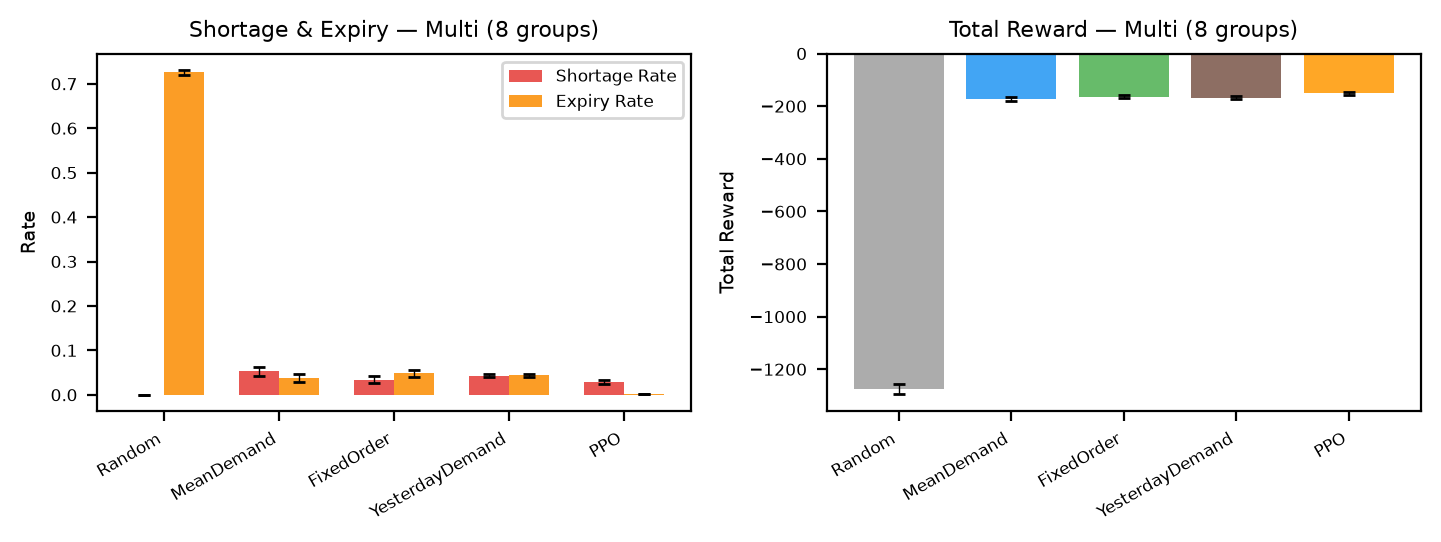
\includegraphics[width=0.9\linewidth]{../figures/compare_multi.png}
\caption{Multi-group shortages, expiry, and reward.}
\label{fig:compare_multi}
\end{figure}

\begin{figure}[!t]
\centering
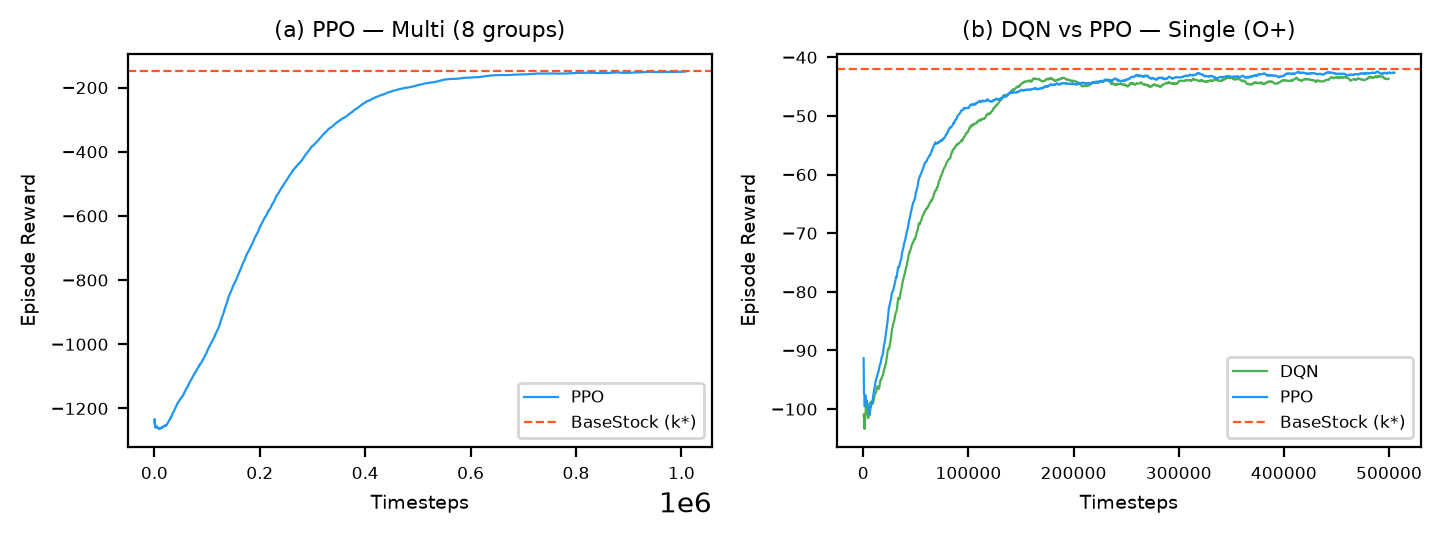
\includegraphics[width=0.9\linewidth]{../figures/learning_curves.png}
\caption{Training rewards; dashed lines show base-stock means.}
\label{fig:learning}
\end{figure}

\begin{figure}[!t]
\centering
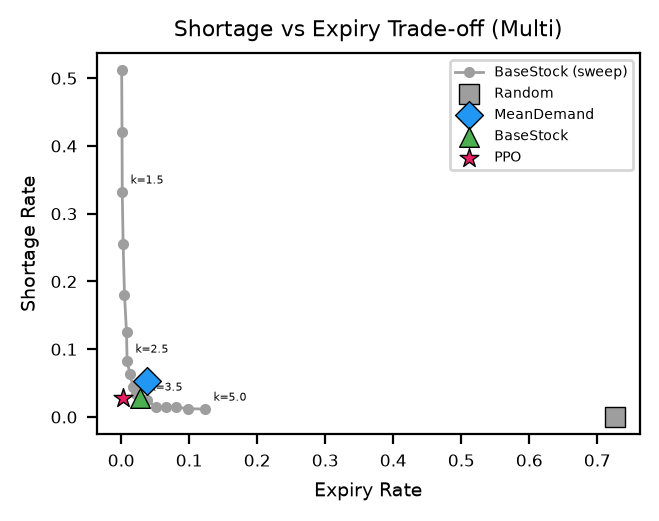
\includegraphics[width=0.55\linewidth]{../figures/tradeoff.png}
\caption{Multi-group shortage--expiry trade-off.}
\label{fig:tradeoff}
\end{figure}

\subsection{Discussion and Limitations}

The final multi-group PPO nearly matches base-stock reward while reducing expiry (0.21\% vs. 2.81\%); base-stock retains a slightly better mean reward. Longer single-group PPO is close to base-stock, while DQN is slightly worse. In the seed-1000 trace, PPO lowered shortages for O$-$, A$-$, and B$-$ but raised them for AB$+$. Its Saturday/Sunday shortage rates were also higher than base-stock in that trace, so no weekend advantage is established. Substitution shares compatible surplus across groups, but no ablation isolates its contribution. These subgroup and weekday observations come from one seed. Demand is synthetic~\cite{abouee2023platelet,uclh2024platelet}; lead time and compatibility are simplified.
